\documentclass[letterpaper,12pt]{article}
\usepackage[utf8]{inputenc}

\usepackage{rotating}
\usepackage[top=1in, bottom=1in, left=1in, right=1in]{geometry}
\usepackage{graphicx}
\usepackage[numbers,square,sort&compress]{natbib}
\usepackage{setspace}
\usepackage[cdot,mediumqspace,]{SIunits}
\usepackage{hyperref}
\usepackage{mathtools}
\usepackage{url}
\usepackage{authblk}
\usepackage{placeins}
\usepackage{float}

\onehalfspacing
\title{Astrometric Orbit Determination }
\author{Anita Bahmanyar \qquad Ayushi Singh \qquad Morten Nyborg Stostad \\Department of Astronomy and Astrophysics, University of Toronto}
\affil{\small {Written by: Anita Bahmanyar}}
\affil{\small {anita.bahmanyar@mail.utoronto.ca}}
\affil{\small {Student Number: 998909098}}
%\affil{\small {anita.bahmanyar@mail.utoronto.ca}}
\date{February 3, 2014}

\usepackage{graphicx}

\begin{document}

\maketitle

%Abstract
\begin{abstract}
\label{abstract}
Astrometry is used to measure properties of celestial objects such as their position on the sky, their movement, velocities and acceleration. In this experiment, we used a charged coupled device called CCD that mapped the sky on a 2D plane. Observations were made using the Dunlap Institute Telescope located in New Mexico, United States. The object of interest for this experiment is an asteroid named 30 Urania.We measured the plate constants of the CCD in order to correct for the non-ideal CCD. Then we applied these plate constants to the data from 30 Urania over the course of four nights in January 2012 and measured the corresponding right ascension and declination of this asteroid in order to determine the orbit of motion of the asteroid and to find its orbital elements such as the inclination, its true, mean and eccentric anomaly, its semi major axis and .



\end{abstract}

%Introduction
\section{Introduction}
\label{sec:introduction}
Nowadays, with the advancements of technology, we are able to use computers to do astrometry in order to obtain position and motion of celestial objects. We have used the stellar map of NGC7331 taken with DIT and found the centroid points and compared and matched them with USNO-B1.0 catalogue in order to find the plate constants of the CCD using least square fitting technique. Here in this lab, we will be using the celestial coordinates(\begin{math} \alpha \end{math} and \begin{math} \delta \end{math}) obtained by the conversion from plate constants which is calculated separately for each night(for more precision) in order to find the orbital elements of the asteroid 30 Urania, calculate its distance relative to the Earth and the Sun and to determine its orbit for future time.


%Observation and Data
\section{Observation and Data}
\label{sec:observationanddata}
\subsection{Equipment}
We used the Dunlap Institute Telescope(DIT) which is a 50-cm robotic telescope dedicated to search for optical counterparts of gamma-ray bursts. The telescope was located at New Mexico on Mt. Joy(32:54:10 N +105:31:46 W). The telescope is equipped with a 4096 \begin{math}\times\end{math} 4096 pixel CCD array and the resultant field of view is approximately 36 \begin{math}\times\end{math} 36 arc minutes. Pixel size of this CCD is 9?. This CCD operated in binning mode to collect the data we will be using through this experiment. Binning is useful since it reduces the size of the resultant FITS file and reduces the effect of read-out noise. For 2 \begin{math}\times\end{math} 2 binning the resultant array is 2048 \begin{math}\times\end{math} 2048 pixels.

\subsection{CCD Calibration}
In order to have good images from the CCD we need to calibrate them. A good image is one that is dark subtracted and divided by flat frames. Therefore, in order to use the data from the CCD, we subtracted the dark data from the actual data. Dark data was taken with the same exposure time as the actual data while the shutter was closed. Dark current is produced due to the noise in the CCD and it might come from the thermal energy of the electrons; therefore, CCDs are kept in cool places in order to reduce the noise. We also divided the dark subtracted data by the flat frames. Flats are morning and evening twilight sky images that are used to normalize the image. Another factor to consider are the bias frames, which are zero second exposures that provide a measure of digital offset when the signal is zero. Here, the bias is assumed to be zero for this long exposure with DIT.



% Calculation and Modeling
\section{Calculation and Modeling}
\subsection{Asteroid Position}
The coordinates of astronomical objects are usually measured by the angles right ascension,\begin{math}\alpha \end{math} and declination, \begin{math} \delta \end{math}, in the equatorial system defined by reference stars measured in International Celestial Reference System, taken at epoch 2000. Therefore, the cartesian coordinates are give by equation 1 below.

\begin{equation}
x_{eq}=\cos\alpha \cos\delta, 
y_{eq}=\sin\alpha \cos\delta ,  
z_{eq}=\sin\delta
\end{equation}

We can convert the equatorial coordinate to ecliptic coordinate by a transformation along x-axis by the angle \begin{math} \epsilon \end{math} by equation 2 given below.

\begin{equation}
s=
\begin{pmatrix}
  x \\
  y \\
  z
 \end{pmatrix} 
  =
\begin{pmatrix}
1 & 0 & 0 \\ 
 0 & cos\epsilon & sin\epsilon\\ 
 0 & -sin\epsilon & cos\epsilon
\end{pmatrix}
\begin{pmatrix}
  x_{eq} \\
  y_{eq} \\
  z_{eq}
\end{pmatrix} 
\end{equation}

where \begin{math}\epsilon\end{math} = 23\begin{math} ^{\circ} \end{math}.43929111 is the tilt of the Earth for the equinox 2000. s is in the ecliptic Cartesian frame.
In this manner, we are able to calculate the \begin{math}s_{1}\end{math}, \begin{math}s_{2}\end{math} and \begin{math}s_{3}\end{math} vectors and thereafter, we can calculate the first and second derivatives of \begin{math} s_{2} \end{math} vector by equations 3 and 4 respectively, which are derived by Taylor series approximation method. \begin{math} \tau_{1} \end{math} is the time difference between the second and first observation and \begin{math} \tau_{3} \end{math} is the time difference between the third and second observation.


% s2 dot equation
\begin{equation}
\dot{s_{2}}=\frac{\tau_{3}(s_{2}-s_{1})}{\tau_{1}(\tau_{1}+\tau_{3})}+\frac{\tau_{1}(s_{3}-s_{2})}{\tau_{1}(\tau_{1}+\tau_{3})}
\end{equation}


% s2 dot dot equation
\begin{equation}
\ddot{s_{2}}=\frac{2(s_{3}-s_{2})}{\tau_{3}(\tau_{1}+\tau_{3})}+\frac{2(s_{2}-s_{1})}{\tau_{1}(\tau_{1}+\tau_{3})}
\end{equation}

The next step is to find the {\bf R} vector. We obtain the components of the {\bf R} vector from the JPL Horizons Ephemeris web interface for the desired date which is 24th, 25th and 26th of January 2012.
The {\bf R} vector components are given in the table 1.






%Table showing the R vector components 
\FloatBarrier
\begin{table}[h!]
\caption{Sun-Earth vector Cartesian components of {\bf R} in ecliptic coordinates [Au]} % title of Table
\centering % used for centering table
\begin{tabular}{| c | c | c |} % centered columns (4 columns)
\hline %inserts double horizontal lines
X & Y & Z \\ [0.5ex] % inserts table
%heading
\hline % inserts single horizontal line
-0.4820742567460204  & 0.8578010618775774  &  -2.425231096584922 \begin{math} \times \end{math}10^{-5} \\ \hline
-0.4974148410812385  & 0.8490994851434150  &  -2.462584044959891 \begin{math} \times \end{math}10^{-5} \\ \hline
-0.5280130493076013  & 0.8306420761670466  &  -2.515673232526080 \begin{math} \times \end{math}10^{-5} \\  \hline
-0.5419538025371889  & 0.8217251214639645  &  -2.524538626668697 \begin{math} \times \end{math}10^{-5}  \\ [1ex] % [1ex] adds vertical space
\hline %inserts single line
\end{tabular}
\label{table:nonlin} % is used to refer this table in the text
\end{table}
\FloatBarrier


%Table showing right ascension and declination
\FloatBarrier
\begin{table}[h!]
\caption{Date and position of asteroid 30 Urania obtained by conversion from plate constants} % title of Table
\centering % used for centering table
\begin{tabular}{| c | c | c | c |} % centered columns (4 columns)
\hline %inserts double horizontal lines
UT Date 2012/01 & Julian Date & Right Ascension(radians) & Declination(radians) \\ [0.5ex] % inserts table
%heading
\hline % inserts single horizontal line
19   &   2455946.68646  & 0.77589496  &  0.33553406  \\ \hline
20   &   2455947.69476  & 0.77991461  &  0.33640024  \\ \hline
22   &   2455949.73866 &  0.78825718 &   0.33765579  \\  \hline
23   &   2455950.68528  & 0.79249126 &   0.33851884  \\ [1ex] % [1ex] adds vertical space
\hline %inserts single line
\end{tabular}
\label{table:nonlin} % is used to refer this table in the text
\end{table}
\FloatBarrier



%Table showing right ascension and declination obtained from JPL
\FloatBarrier
\begin{table}[h!]
\caption{Date and position of asteroid 30 Urania in the sky obtained from JPL} % title of Table
\centering % used for centering table
\begin{tabular}{| c | c | c | c |} % centered columns (4 columns)
\hline %inserts double horizontal lines
UT Date 2012/01 & Julian Date & Right Ascension(radians) & Declination(radians) \\ [0.5ex] % inserts table
%heading
\hline % inserts single horizontal line
19   &   2455946.68646  & 0.775884664&   0.335833345 \\ \hline
20   &   2455947.69476  & 0.779874196  & 0.33648493   \\ \hline
22   &   2455949.73866 &  0.788401584 & 0.337913196    \\  \hline
23   &   2455950.68528  &  &     \\ [1ex] % [1ex] adds vertical space
\hline %inserts single line
\end{tabular}
\label{table:nonlin} % is used to refer this table in the text
\end{table}
\FloatBarrier

Tables 2 and 3 show the position of the asteroid 30 Urania obtained by conversion from plate constants as it has been discussed in lab 3 and the position obtained from JPL HORIZONS, respectively.

We also need to find the magnitude of the R vector for the second data(since the second night is the one we use to find the position of the asteroid as we need three sets of data for figuring out the position). {\bf R} vector magnitude can be calculated by squaring each of the components and taking the square root of their sum as shown in equation 5.

\begin{equation}
R=\sqrt{R_{x}^2+R_{y}^2+R_{z}^2}
\end{equation}


We now have all the values we need and should be able to calculate \begin{math} \rho \end{math} value by the equation 6:

\begin{equation}
\rho=k^2(\frac{1}{R^3}-\frac{1}{r^3})\frac{\dot{{\bf s}}.({\bf R}\times{\bf s})}{\dot{{\bf s}}.(\ddot{{\bf s}}\times{\bf s})}
\end{equation}

We do not have the value or r explicitly yet; however, we can guess an initial r value and write a for loop to calculate \begin{math} \rho \end{math} until it converges using the new values for r. This part of the code I used can be found in the appendix.(....)


After finding the \begin{math} \rho \end{math} value, we can calculate the r value by equation 7:

\begin{equation}
r^2=\rho ^2 + R^2 + 2\rho {\bf R}. {\bf s}
\end{equation}

Note that this r is different from the one we just guessed in equation 6. 
We can also calculate derivative of \begin{math} \rho \end{math} using equation 8 :
\begin{equation}
\dot{\rho}=\frac{k^2}{2}(\frac{1}{{\bf R}^3}-\frac{1}{r^3})\frac{\ddot{s}.({\bf R}\times {\bf s})}{\ddot{{\bf s}}.({\bf \dot{s}}\times {\bf s})}
\end{equation}

We can now calculate the position vector of the asteroid with respect to sun using simple vector addition:

\begin{equation}
{\bf r}= {\bf R}+r{\bf s}
\end{equation}
We may also find the derivative of the {\bf R} vector using the same way we found the derivative of the vector {\bf s}, which can be written as equation 10:

\begin{equation}
\dot{{\bf R_{2}}}=\frac{\tau_{3}({\bf R_{2}}-{\bf R_{1}})}{\tau_{1}(\tau_{1}+\tau_{3})}+\frac{\tau_{1}({\bf R_{3}}-{\bf R_{2}})}{\tau_{1}(\tau_{1}+\tau_{3})}
\end{equation}

In order to calculate the velocity of the asteroid relative to the sun we need to find the derivative of the {\bf r} vector we found in equation 9 and employ equation 11:

\begin{equation}
{\bf \dot{r}}={\bf \dot{R}} +\rho{\dot{\bf s}} + \dot{\rho} {\bf s}
\end{equation}




%Table showing r_vector and r_dot values 
\FloatBarrier
\begin{table}[h!]
\caption{Derived Geocentric Sun-asteroid vector and its time derivative. The Cartesian components are given in the heliocentric ecliptic system.} % title of Table
\centering % used for centering table
\begin{tabular}{| c | c | c | c |} % centered columns (4 columns)
\hline %inserts double horizontal lines
Vector & x & y & z \\ [0.5ex] % inserts table
%heading
\hline % inserts single horizontal line
{\bf r}  & 0.58976309  &  2.0483579709 &  0.062989112\\ \hline
\begin{math} {\bf \dot{r}} \end{math} & -0.01171778  &  0.00405553 &  -0.00024878 \\  [1ex] % [1ex] adds vertical space 
\hline %inserts single line
\end{tabular}
\label{table:nonlin} % is used to refer this table in the text
\end{table}
\FloatBarrier

Table 4 shows the r vector and its derivative Cartesian components in the heliocentric ecliptic system.

% Orbital Elements Sub Section
\subsection{Orbital Elements}
We can now use the values we got from previous section to find the orbital elements of 30 Urania using Laplace's method. Since we know the magnitude of the radius vector, r, the asteroid velocity, \begin{math}V=|\dot{r}| \end{math} and k=0.017202098950, we can compute the semi-major axis by equation 12:

% Semi Major Axis Equation
\begin{equation}
a=\frac{k^2r}{2k^2-rV^2}
\end{equation}

Then we can compute the {\bf h} vector components by the cross product of the {\bf r} and {\bf \dot{r}} vectors:
\begin{equation}
{\bf h}= {\bf r} \times {\bf \dot{r}}
\end{equation}
Using the {\bf h} vector components, we can compute \begin{math} \Omega \end{math} and i by equations 14 and 15 respectively:

% Omega orbital element
\begin{equation}
\tan \Omega = \frac{-h_{x}}{h_{y}}
\end{equation}

% i orbital element
\begin{equation}
\cos i = \frac{h_{z}}{h}
\end{equation}

In order to find the eccentricity, we use equation 16 given below:

% eccentricity orbital element
\begin{equation}
e=\sqrt{1-(\frac{h^2}{ak^2})}
\end{equation}

In order to compute the last two Keplerian orbital elements-the argument of perihelion,\begin{math} \omega \end{math}, and the epoch of perihelion, \begin{math} \tau \end{math}, we need to calculate the eccentric and true anomalies. Equation 17 and 18 give the eccentric and true anomalies, respectively.

% eccentric anomaly orbital element
\begin{equation}
\cos E = \frac{a-r}{ae}
\end{equation}

The sign of E depends on the body's radial velocity; E>0 when the radial velocity is positive(between perihelion and aphelion) and E<0 when the radial velocity is negative(from aphelion to perihelion).

% True Anomaly Equation
\begin{equation}
v = 2\arctan(\sqrt{\frac{1+e}{1-e}\tan E/2})
\end{equation}

% true anomaly orbital element
\begin{equation}
\cos (v+\omega) = \frac{x \cos \Omega + y \sin \Omega}{r} 
\end{equation}


For the epoch of perihelion, \begin{math} \tau \end{math} we can use equation 20 :

% Mean Anomaly Equation
\begin{equation}
M = n(t-\tau)
\end{equation}
where \begin{math} n=ka^-3/2 \end{math} is the mean motion and t is the epoch of the second observation. The calculated orbital elements of the asteroid Ceres are listed in table 5 along with their true values and the error in each. Since the error is small, we can be confident about our method and values. However, during this lab we found out that this method is very sensitive to the coordinates of the asteroid obtained via transformation by plate constants. At first, we were using values that were similar to the true values (JPL values) within two decimal places, but the values of {\bf r} and \begin{math} \rho \end{math} were converging to 0 and 1 respectively, which meant that the asteroid is somewhere on the surface of the Earth. After computing more accurate right ascension and declination of the asteroid using more precise plate constants with smaller \begin{math} \chi_{reduced}^2 \end{math}, the values of the RA and Dec of the asteroid matched with the JPL values within 4 decimal places and we were able to get good estimate of the position of the asteroid.
In order to make sure that our method and equations are correct, we first applied the same method and equations to the asteroid Ceres and compared the orbital elements we got with the ones given in the lab handout and they matched with small residuals; therefore, we were confident about the method and the equations used to compute the orbital elements of 30 Urania.

%Table showing the R vector components 
\FloatBarrier
\begin{table}[h!]
\caption{Orbital Elements of Ceres obtained by our calculations and JPL along with their errors} % title of Table
\centering % used for centering table
\begin{tabular}{| c | c | c | c | c | c | c |} % centered columns (4 columns)
\hline %inserts double horizontal lines
 & a & \begin{math} \Omega \end{math}  & i & e & \begin{math} \omega \end{math}  & \begin{math} \tau \end{math} \\ [0.5ex] % inserts table
%heading
\hline % inserts single horizontal line
  & [Au]  &  [deg] &[deg] & & [deg] & [Julian Date] \\ \hline 
True & 2.766 &  80.72 &   10.61 & 0.179 & 73.12 &2454785.970\\ \hline
Estimated &3.186 &  80.68 & 10.50 &  0.079 & 62.51 & 2454868\\  \hline
Error & -0.42 &  0.04 &    0.11 &   0.09 & 10.61 & 82.03\\[1ex] % [1ex] adds vertical space
\hline %inserts single line
\end{tabular}
\label{table:nonlin} % is used to refer this table in the text
\end{table}
\FloatBarrier

% Orbital Motion of the Asteroid Ceres
\subsection{Orbital Motion of Asteroid Ceres}
In this sub section, we will be using Keplerian orbital elements provided in the lab handout to compute and plot some of the orbital elements such as true anomaly and the orbital separation, r, as a function of time. 
We first need to compute the mean anomaly given by equation 21. Then using Taylor series we are able to find the \begin{math} E_{n} \end{math} numerically by the following equation:

% Eccentric Anomaly 
\begin{equation}
E_{n+1}=E_{n}+\frac{M-M(E_{n})}{1-e\cos(E_{n})}
\end{equation}


We can then plot the eccentric and true anomalies as a function of time in Julian Date. The result is shown in figure 1.

% Figure 3 in lab handout
\FloatBarrier
\begin{figure}[h!]
\centering
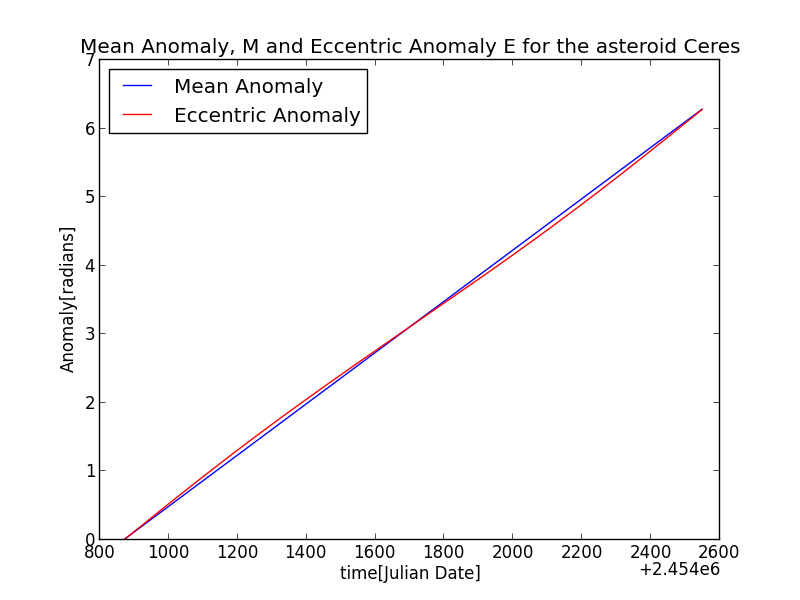
\includegraphics[scale=0.5]{figure3.png}
\caption{This figure shows the mean anomaly, M, and eccentric anomaly, E, for the asteroid Ceres using the orbital elements tabulated in table 5. The eccentricity of Ceres is small(e=0.079) and the difference between these two angles is small.}
\end{figure}
\FloatBarrier


We can then compute the true anomaly by equation 18 and since we have both \begin{math} v \end{math} and \begin{math} w \end{math} , we are able to calculate the polar angle by equation 22

\begin{equation}
\theta = v + \omega
\end{equation}

and the Cartesian components of the position of the asteroid are given by equation 23:

\begin{equation}
r=
\begin{pmatrix}
  r\cos \theta \\
  r\sin \theta \\
  0
 \end{pmatrix} 
\end{equation}

The plot of the orbital separation, r, and the true anomaly, \begin{math} v \end{math}, as a function of time are shown in figure 2:
% figure 2
\FloatBarrier
\begin{figure}[h!]
\centering
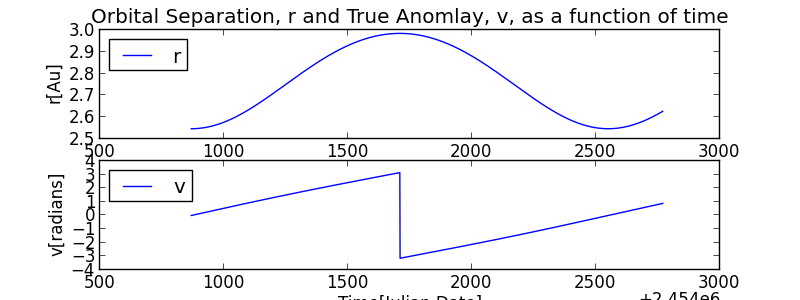
\includegraphics[scale=0.4]{figure4.png}
\caption{This figure shows the orbital separation and true anomaly of the asteroid Ceres respectively over one period.}
\end{figure}
\FloatBarrier



% figure 3
\FloatBarrier
\begin{figure}[h!]
\centering
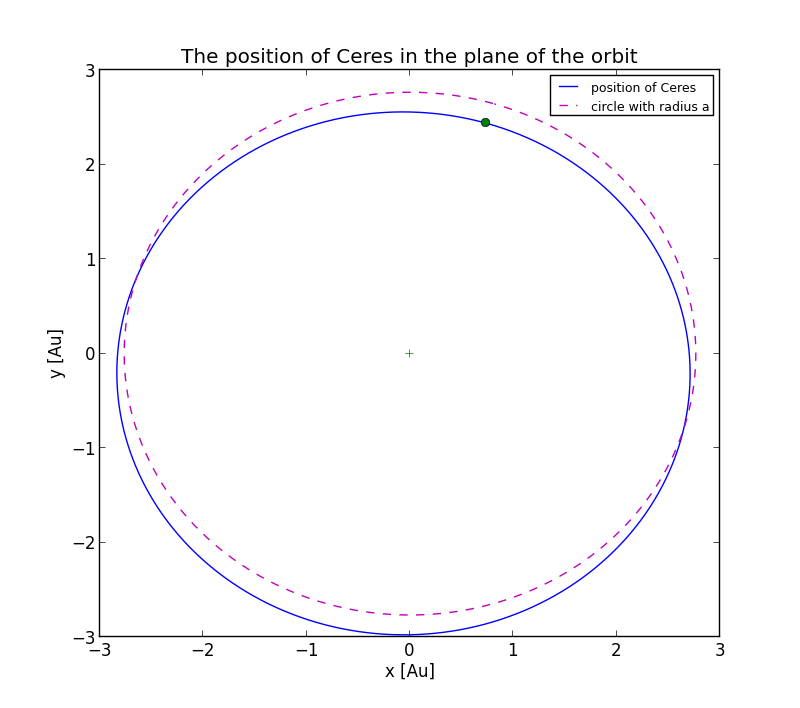
\includegraphics[scale=0.4]{figure5.png}
\caption{This figure shows the x and y components of r vector for asteroid Ceres. The pink dashed line is a circle with radius equal to the semi-major axis of Ceres and the blue solid line is the orbit of Ceres. The position of perihelion is also pointed with a dot.}
\end{figure}
\FloatBarrier



% Orbital Motion of the Asteroid 30 Urania
\subsection{Orbital Motion of Asteroid 30 Urania}
The same way we predicted the position of Ceres for future time, we can determine the orbit of motion of 30 Urania using the orbital elements we computed in the previous sections. Table 6 contains the orbital elements of 30 Urania computed, the elements obtained from JPL HORIZONS and the error in our values.


%Table showing the orbital elements of 30 Urania 
\FloatBarrier
\begin{table}[h!]
\caption{Orbital Elements of 30 Urania obtained by our calculations and JPL along with their errors.} % title of Table
\centering % used for centering table
\begin{tabular}{| c | c | c | c | c | c | c |} % centered columns (4 columns)
\hline %inserts double horizontal lines
 & a & \begin{math} \Omega \end{math}  & i & e & \begin{math} \omega \end{math}  & \begin{math} \tau \end{math} \\ [0.5ex] % inserts table
%heading
\hline % inserts single horizontal line
  & [Au]  &  [deg] &[deg] & & [deg] & [Julian Date] \\ \hline 
True & 2.365 & 307.93  &  2.099  & 0.127 &  86.277 & 2455833.107\\ \hline
Estimated & 2.133 &  307.75 & 2.11 &  0.125 & 87.70 & 2455835.546 \\ \hline
Error & 0.232 & 0.18  &  0.11   &  0.002  & -1.42 & -2.439\\[1ex] % [1ex] adds vertical space
\hline %inserts single line
\end{tabular}
\label{table:nonlin} % is used to refer this table in the text
\end{table}
\FloatBarrier

We can then determine the orbit of 30 Urania using these orbital elements. The Cartesian components of r of this asteroid in ecliptic coordinate could be obtained by equation 24, where \begin{math} \theta = \nu + \omega \end{math}:

\begin{equation}
s=
\begin{pmatrix}
  x \\
  y \\
  z
 \end{pmatrix} 
  =r
\begin{pmatrix}
\cos \Omega \cos \theta - \sin \Omega \cos i \sin \theta \\ 
 \sin \Omega \cos \theta+ \cos \Omega \cos i \sin \theta \\ 
 \sin i \sin \theta
\end{pmatrix}
\end{equation}

We need the values of true and eccentric anomalies at different times, so we must iteratively solve for E using Newton?s method given in equation 21, where we used \begin{math} E_{0}=M \end{math}. We can also plot the mean and eccentric anomalies as a function of time for 30 Urania as it is shown in figure 4.



% figures 4 and 5
\begin{figure}[ht]
\centering
\begin{minipage}[b]{0.4\linewidth}
  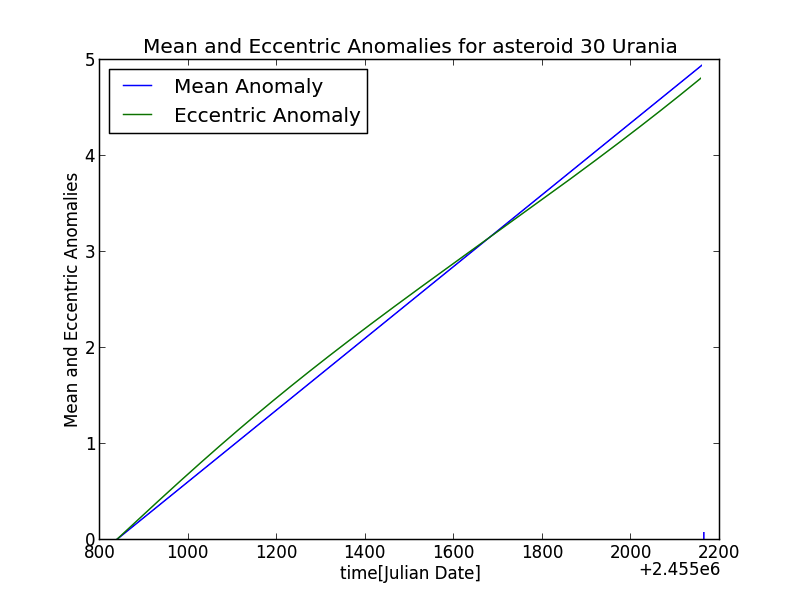
\includegraphics[scale=0.25]{mean_eccentric_urania.png}
  \caption{This figure shows the mean and eccentric anomalies of asteroid 30 Urania. Even though the values fluctuate, the values are very close to each other. This is due to the small eccentricity we found for 30 Urania.}
  \label{fig:minipage1}
\end{minipage}
\quad
\begin{minipage}[b]{0.4\linewidth}
  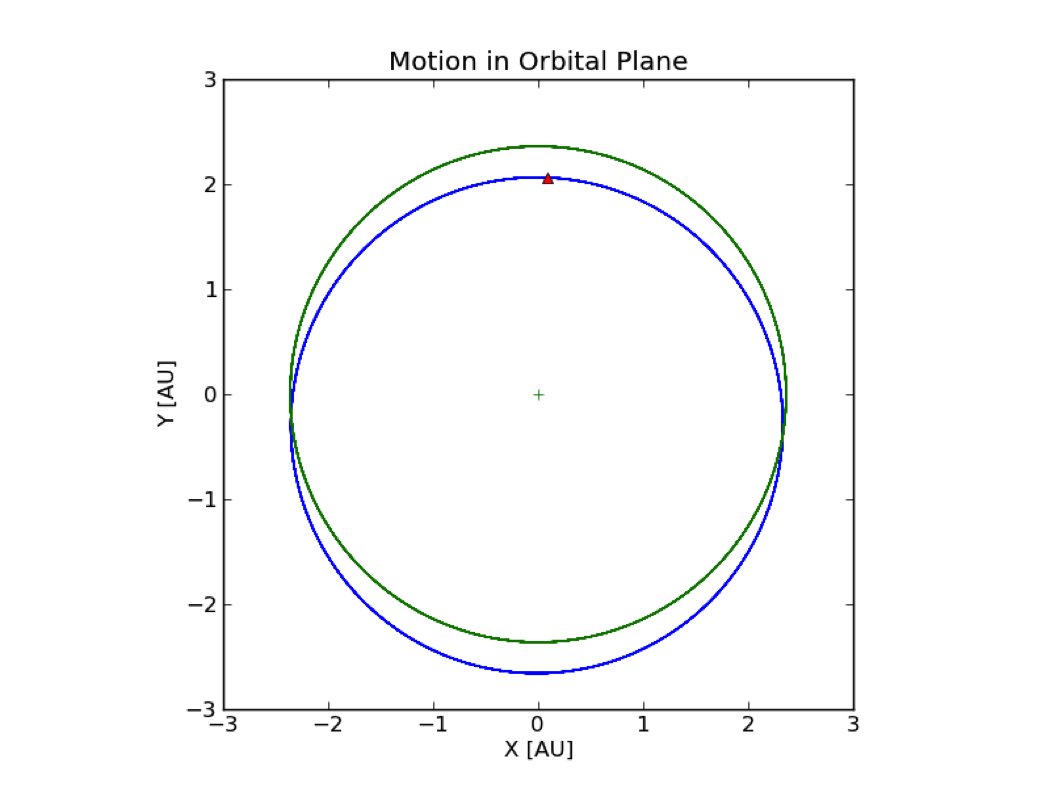
\includegraphics[scale=0.4]{orbit_urania.png}
  \caption{This figure shows a circle with radius equal to semi-major axis of 30 Urania (green line)and its true orbit(blue line). This also shows the location of the perihelion of this asteroid pointed by a red triangle.}
  \label{fig:minipage2}
\end{minipage}
\end{figure}





We can then use the transpose of matrix 2 in order to transform the ecliptic coordinates to the equatorial coordinated by equation 25. We can then find the values of \begin{math} \alpha \end{math} and \begin{math} \delta \end{math} using equations 26 and 27, respectively.s
% equatorial transformation
\begin{equation}
\begin{pmatrix}
  x_{eq} \\
  y_{eq} \\
  z_{eq}
 \end{pmatrix} 
  =
\begin{pmatrix}
1 & 0 & 0 \\ 
 0 & cos\epsilon & -sin\epsilon\\ 
 0 & sin\epsilon & cos\epsilon
\end{pmatrix}
\begin{pmatrix}
  x \\
  y \\
  z
\end{pmatrix} 
\end{equation}



%  equations 66
\begin{equation}
\tan \alpha= \frac{y_{eq}}{x_{eq}}
\end{equation}
\begin{equation}
\sin \delta= z_{eq}
\end{equation}


% Discussion
\section{Discussion}
\label{sec:discussion}
First of all, we tried to compute the geocentric position vector of the asteroid, \begin{math} \rho \end{math}s, and the relative position of the asteroid relative to the Sun,{\bf r}, using the equations 1 to 11. In computing the positions, we used the position vector of the Earth relative to the Sun, {\bf R}=\begin{math} (X_{eq},Y_{eq},Z_{eq})\end{math}, obtained from JPL HORIZONS ephemeris for the given date. Hence, we could determine the orbit of the asteroid using Laplace's method which is explained in section 4 in details. In order to determine the position of the asteroid relative to the Sun, we also needed the right ascension and declination of the asteroid in the course of the four epochs of the observations we had from the DIT files. As it has been mentioned in the report and has been mentioned in full details in my lab 3 report, we calculated the plate constants of the CCD used in order to correct for the non-ideal CCD and to obtain more accurate positions of the asteroid on the celestial sphere. However, we faced lots of problems and we were getting \begin{math} \rho \end{math} to be zero and {\bf r} to be almost 1, which meant that the asteroid is 1 Au away from the Sun and 0 Au away from the Earth which meant the asteroid is on the Earth! Therefore, we tried to fix the problem, so we used more accurate Julian dates (with more precision) and also used different epochs. For instance, we used the first, second and third epoch and then we used second, third and fourth epoch to compute \begin{math} \rho \end{math} and {\bf r}, but it did not solve the problem. The other thing we used was to use the coordinates (\begin{math} \alpha \end{math} and \begin{math} \delta \end{math})obtained from JPL to check if there is a problem with the code itself or with the coordinates we were using and we found out that the code works perfectly. The values we got for \begin{math} \rho \end{math} and {\bf r} were really close to the true values. The values we had from our conversion using the plate constants were very close to the true values obtained from JPL, they were the same to 4 decimal places; however, as we saw, the calculation of the position vectors is very sensitive to the precision in the \alpha \end{math} and \begin{math} \delta \end{math} values. 


% Conclusion
\section{Conclusion}
\label{sec:conclusion}
We used 2D images of 30 Urania to compute its orbital elements in order to predict its orbit for future dates. We used the coordinates obtained by conversion from CCD pixels to right ascension and declination using plate constants of the CCD for each night;however, since our values differed from the true values in 4th decimal place, we used values obtained from JPL HORIZONS web interface. Therefore, we observed that we need very accurate positions of the asteroid since only this small difference can make a huge difference in the orbital elements and as a result, in the prediction of the asteroid's orbit.

% Reference
\section{References}
\label{sec:references}
\\*1- Lab # 4: Astrometric Orbit Determination handout
\\*2- Lab 3 Report written by Anita Bahmanyar
\\*3-JPL HORIZONS web interface ephemeris

\section{Appendix}
\label{sec:appendix}
Here is a it of my code to calculate the mean and eccentric anomaly iteratively, using equations 20 and  21:
M[q-1] and E[q-1] are the (q-1)th values of mean and eccentric anomalies. 
for q in range(1,len(t)):

\\       M[q-1]=E[q-1]-e*(np.sin(E[q-1]))
\\       E[q]=E[q-1]+((mu[q-1]-M[q-1])/(1-e*np.cos(E[q-1]))) 
   
This loops starts from one and continues until it is smaller than the number of elements in time array and calculates the mean anomaly for each time it goes into the loop and using that specific M value, it computes the E value. We should also note that the initial values of E[0]=mu[0] and M[0]=E[0], where mu=n*(t-tau) and t is the time array starting from tau=2454868; therefore, mu[0]=0.
    

\\for plotting figure 3, I used the following code, where \begin{math} circle_x \end{math} and \begin{math} circle_y \end{math}are the components of a circle with radius equal to semi-major axis of Ceres and \begin{math} r_x \end{math} and \begin{math} r_y  \end{math} are the components of Ceres's orbit:
\\circle_x=a*(np.cos(theta))
\\circle_y=a*(np.sin(theta))
 and 
\\r_x=r*(np.cos(theta))
\\r_y=r*(np.sin(theta))


\\Then I used a for loop to run for 20 times in order to find the \begin{math} \rho \end{math} and r values close to the true values. This loop goes until the value of r and \begin{math} \rho \end{math} we have found, converge to their true values:

for i in range(20):

rho=((k**2)*((1./(R-length**3))-(1./(r1**3))))*denom

r1=np.sqrt((rho**2)+(R-length**2)+(2*rho*R-dot_-))
    
\\Where denom=(sdot-R-s)/(sdot-s-dotdot-s).

Here are also calculation of some of the orbital elements:

a-theory=((k**2)*r1)/((2*(k**2))-(r1*(V**2)))       ,        semi-major axis, a

np.cross(r-vector,dr-dt)        ,       h vector which is the cross product of r vector and its derivative

big-omega=((np.arctan(h[0]/h[1]))*180)/(np.pi)        ,     \begin{math} \Omega \end{math}


 

%\FloatBarrier
%\begin{figure}[h!]
%\centering
%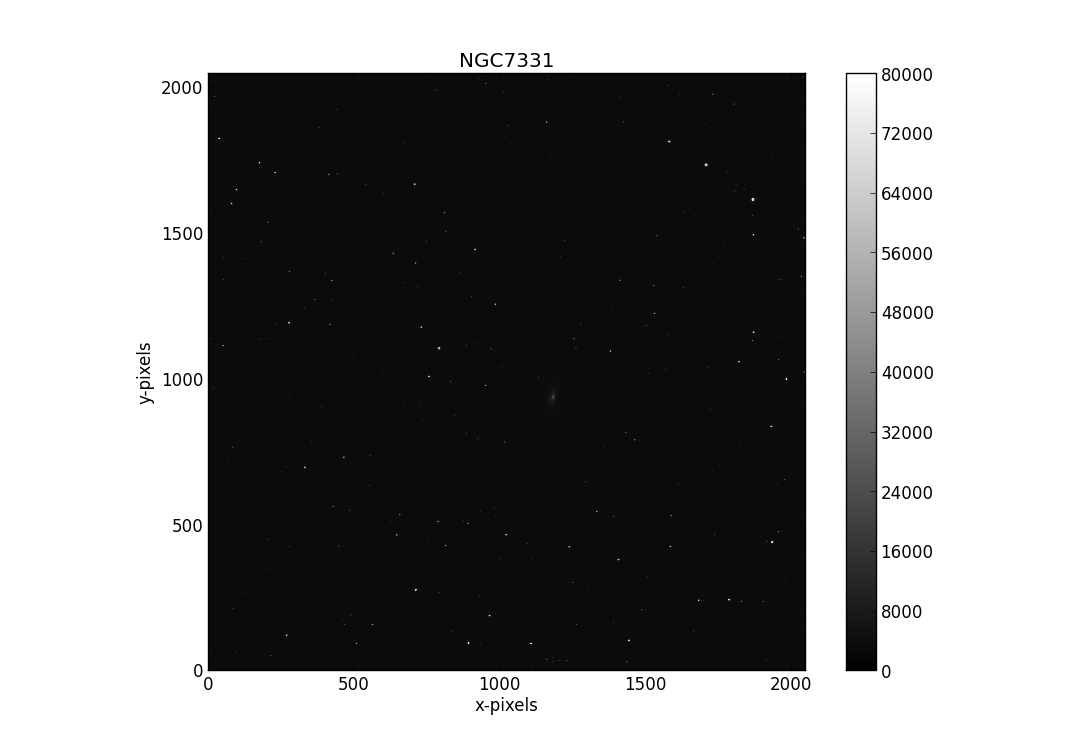
\includegraphics[scale=0.6]{ngc7331.png}
%\caption{This figure shows the NGC7331. The colour bar shows the intensity of the objects with black having zero intensity. This image is dark subtracted and divided by flat in order to be normalized.}
%\end{figure}
%\FloatBarrier

\end{document}


